  %%%%%%%%%%%%%%%%%%%%%%%%%%%%%%%%%%%%%%% -*- coding: utf-8; mode: latex -*- %%
  %
%%%%%                         CHAPTER
 %%%
  %

% $Id: 2300-omnis-iste-natus.tex,v 1.2 2007/11/23 10:14:54 david Exp $
% $Log: 2300-omnis-iste-natus.tex,v $
% Revision 1.2  2007/11/23 10:14:54  david
% Bug fixes galore.
%
% Revision 1.1  2007/11/23 09:52:42  david
% *** empty log message ***
%
%

  %%%%%%%%%%%%%%%%%%%%%%%%%%%%%%%%%%%%%%%%%%%%%%%%%%%%%%%%%%%%%%%%%%%%%%%%%%%%%
  %
%%%%%                     HEAD MATTER
 %%%
  %

\chapter{Namespace Operation Performance Assessment}
%\addcontentsline{lof}{chapter}{\thechapter\quad Irure Dolor}
%\addcontentsline{lot}{chapter}{\thechapter\quad Irure Dolor}
\label{ch:Assessment}

 In this chapter, we will give the namespace operation performance assessment between the second version (we called it PCC version) of Hop-HDFS and original HDFS under single NameNode. All the tests in this chapter are performed under same the experimental testbed described in Chapter~\ref{ch:evaluation} Section~\ref{sec:testbed}.

\section{NameNode Throughput Benchmark}

A \textit{NNThroughtBenchmark}~\cite{shvachko2010hdfs} tool has been developed to measure the NameNode performance. It is included in the Apache HDFS test package. The tool used in this assessment is based on the code from Apache Hadoop HDFS 2.0.4 Aplha (We integrate the part which tests \textit{mkdirs} operation from HDFS 2.3.0 NNThroughtBenchmark into this one).

\noindent \textit{NNThroughtBenchmark} starts a single NameNode and runs multiple client threads on the same node.  The same NameNode operation is performed by each client repetitively via directly calling the implemented method. The number of operations performed by the NameNode per second is measured.

\noindent In this section, we aims to give a performance comparison between HDFS and PCC. Since the workload is generated from a single machine by the \textit{NNThroughtBenchmark}, we set the number of operations to be 100 and the number of threads to be 3. For operations \textit{create, delete and rename}, the total number of files involved is 100. They are placed under 4 different directories equally. For operation \textit{mkdirs}, the total number of directories created is 100 and they are also placed under 4 different directories equally. See Figure~\ref{fig:nntp} for the operation performance comparison between HDFS and PCC.

\begin{figure}[h]
	\centering
	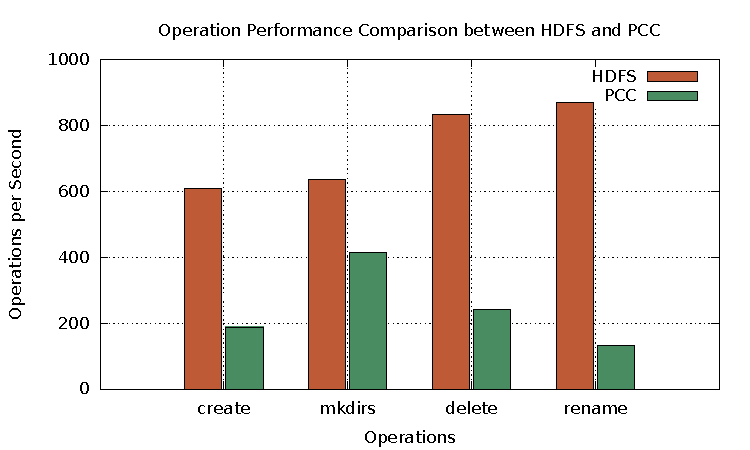
\includegraphics[width=\linewidth]{figs/nn_100.pdf}
	\caption{Operation Performance Comparison between HDFS and PCC}
	\label{fig:nntp}
\end{figure}

\noindent From Table~\ref{table:nntpb}, we find that the throughput of \textit{mkdirs} in PCC is 64.9 \% of HDFS, while others are all less than 30\%. The reason why the performance of \textit{create, delete and rename} is worse is because they involve multiple NameNode primitive operations. For example, to finish the \textit{create} operations, it takes two NameNode primitive operations (two transactions): \textit{startFile} and \textit{completeFile}. Since each NameNode primitive operation is implemented as a single transaction, the more primitive operations involved, the more parent write locks will be, which means that more transactions will be blocked.

\begin{table}[h]
	\centering
	\begin{tabular}{|c|c|c|c|c|}
		\hline
		\textbf{Operations per Second} & \textbf{create} & \textbf{mkdirs} & \textbf{delete} & \textbf{rename} \\ \hline
		HDFS                           & 609             & 636             & 833             & 869             \\ \hline
		PCC                 & 188             & 413             & 242             & 132             \\ \hline
		PCC / HDFS              & 30.9\%          & 64.9\%          & 29.1\%          & 15.2\%          \\ \hline
	\end{tabular}
	\caption{Operation Performance Comparison between HDFS and PCC}
	\label{table:nntpb}
\end{table}

\section{Parent Directory Contention Assessment}
\label{sec:pdcassement}
The worst case in PCC happens when all concurrent operations try to work under the same directory. Even though they mutate different INodes, all handling transactions will put a parent directory write lock to block each other. Therefore, the parent directory becomes a contention point.

\noindent Here we design a test for the parent directory contention assessment. We build a thread pool with size 1024 for clients. We have three tests with 1000, 10000 and 100000 concurrent clients separately. Each client creates (\textit{mkdirs()}) one sub-directory. All these sub-directories are different, but they are all created under the same parent directory. The parent directory is the contention point in each task. We measure the elapsed time to finish all the concurrent creation tasks in each test.

\noindent As we can see from Figure~\ref{fig:hdfsPCCparent} and Table~\ref{table:hdfsPCCparent}, it takes 4 - 5 more times in PCC to finish all these tasks compared to HDFS. However, when the size of concurrent tasks increases, this ratio decreases. Because as mentioned in Section~\ref{subsec:rpc}, under heavy workload, the edit logs in HDFS degrade the NameNode performance. Since there is no edit logging and check pointing part in Hop-HDFS, it works more efficiently than HDFS.

\begin{figure}[h]
	\centering
	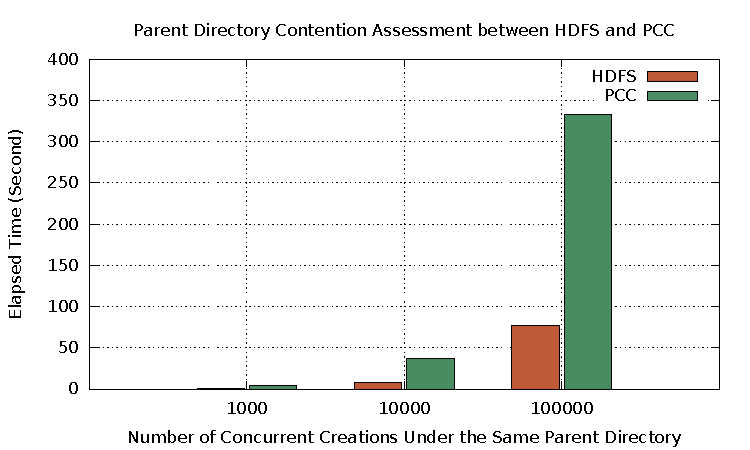
\includegraphics[width=\linewidth]{figs/hdfs_pcc_parentlock.pdf}
	\caption{Parent Directory Contention Assessment between HDFS and PCC}
	\label{fig:hdfsPCCparent}
\end{figure}

\begin{table}[h]
	\centering
	\begin{tabular}{|c|c|c|c|}
		\hline
		\textbf{Num. of Concurrent Creation} & \textbf{1000} & \textbf{10000} & \textbf{100000} \\ \hline
		HDFS                                 & 0.82s         & 7.83s          & 77.13s          \\ \hline
		PCC                       & 4.35s         & 36.74s         & 332.36s         \\ \hline
		PCC / HDFS                           & 530.5\%       & 469.2\%        & 430.9\%         \\ \hline
	\end{tabular}
		\caption{Parent Directory Contention Assessment between HDFS and PCC}
		\label{table:hdfsPCCparent}
\end{table}

\noindent Note that the tests performed in this chapter is based on single NameNode. The multi-NameNode architecture in Hop-HDFS will help to improve the overall throughput.

\section*{Summary}
In this chapter we provided a systematic namespace operation performance assessment between the second version of Hop-HDFS (PCC version) and original HDFS. We found that with single NameNode, the performance on PCC was worse than HDFS, especially on write-write intense workload with parent directory contention point. However, when the size of concurrent tasks increases, this gap became smaller because check pointing and journaling were not needed in Hop-HDFS. But those part degraded the NameNode performance in HDFS.